\chapter{Benchmark configurations}
\label{app:benchmarks}

\begin{figure}[h]
	\centering
	\begin{subfigure}{.2\textwidth}
		\centering
		
\includegraphics[width=.8\textwidth]{imgs/estee/shapes/plain}
		\caption{}
		\label{fig:tg-plain}
	\end{subfigure}%
	\begin{subfigure}{.2\textwidth}
		\centering
		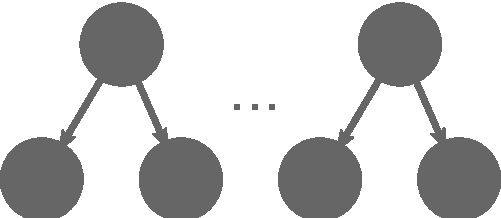
\includegraphics[width=.8\linewidth]{imgs/estee/shapes/fork}
		\caption{}
		\label{fig:tg-fork}
	\end{subfigure}
	\begin{subfigure}{.2\textwidth}
		\centering
		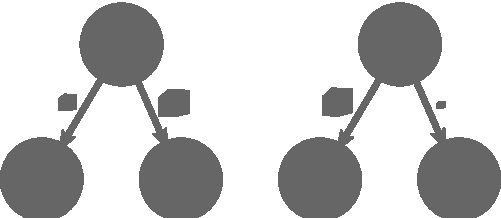
\includegraphics[width=.8\linewidth]{imgs/estee/shapes/fork2}
		\caption{}
		\label{fig:tg-fork2}
	\end{subfigure}
	\begin{subfigure}{.2\textwidth}
		\centering
		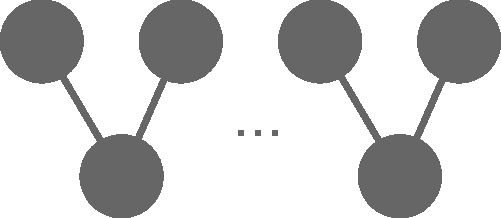
\includegraphics[width=.8\linewidth]{imgs/estee/shapes/v}
		\caption{}
		\label{fig:tg-v}
	\end{subfigure}
	\\
	\begin{subfigure}{.2\textwidth}
		\centering
		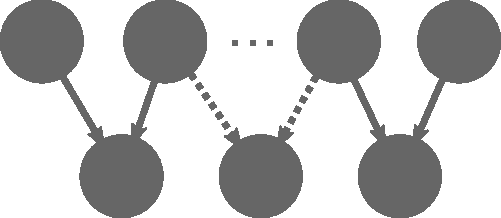
\includegraphics[width=.8\linewidth]{imgs/estee/shapes/w}
		\caption{}
		\label{fig:tg-w}
	\end{subfigure}
	\begin{subfigure}{.2\textwidth}
		\centering
		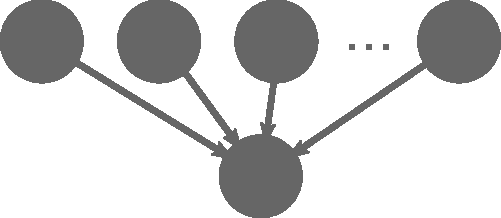
\includegraphics[width=.8\linewidth]{imgs/estee/shapes/merge}
		\caption{}
		\label{fig:tg-merge}
	\end{subfigure}
	\begin{subfigure}{.2\textwidth}
		\centering
		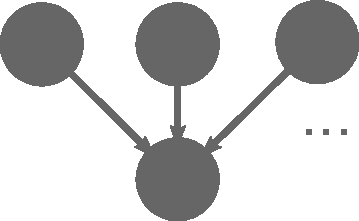
\includegraphics[width=.8\linewidth]{imgs/estee/shapes/merge-triplets}
		\caption{}
		\label{fig:tg-merge-triplets}
	\end{subfigure}
	\begin{subfigure}{.2\textwidth}
		\centering
		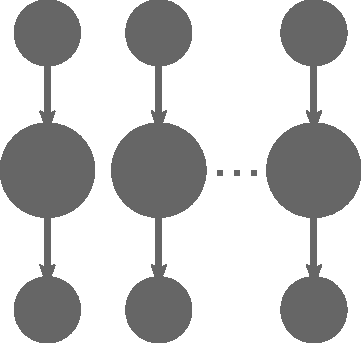
\includegraphics[width=.8\linewidth]{imgs/estee/shapes/triplets}
		\caption{}
		\label{fig:tg-triplets}
	\end{subfigure}
	\\
	\begin{subfigure}{.2\textwidth}
		\centering
		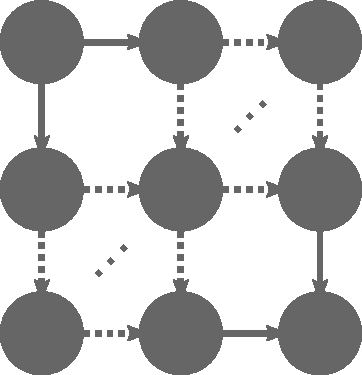
\includegraphics[width=.8\linewidth]{imgs/estee/shapes/grid}
		\caption{}
		\label{fig:tg-grid}
	\end{subfigure}
	\begin{subfigure}{.2\textwidth}
		\centering
		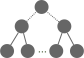
\includegraphics[width=.8\linewidth]{imgs/estee/shapes/splitters}
		\caption{}
		\label{fig:tg-splitters}
	\end{subfigure}
	\begin{subfigure}{.2\textwidth}
		\centering
		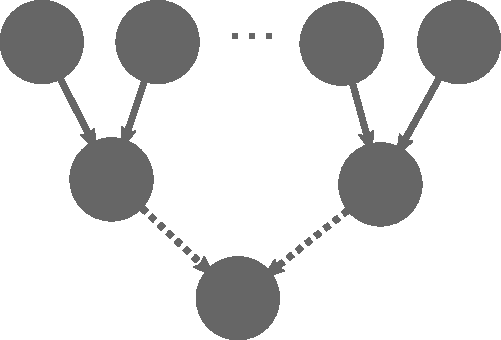
\includegraphics[width=.8\linewidth]{imgs/estee/shapes/conflux}
		\caption{}
		\label{fig:tg-conflux}
	\end{subfigure}
	\begin{subfigure}{.2\textwidth}
		\centering
		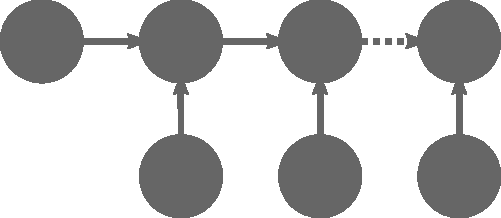
\includegraphics[width=.8\linewidth]{imgs/estee/shapes/fern}
		\caption{}
		\label{fig:tg-fern}
	\end{subfigure}

	\caption{Task graph shapes in the \emph{elementary} \estee{} benchmark data set}
	\label{fig:estee-elementary-shapes}
\end{figure}

\begin{table}[h]
	\centering
	\begin{tabular}{l|lrrrr|T}
		\toprule
		Graph            & D & \#T & \#O   & TS     & LP  & \normalsize{Description}               \\
		\midrule
		plain1n          & e & 380 & 0     & 0.00   & 1   & Independent tasks;
		normally distributed durations (Fig.~\ref{fig:tg-plain})                                   \\
		plain1e          & e & 380 & 0     & 0.00   & 1   & Independent tasks;
		exponentially distributed durations (Fig.~\ref{fig:tg-plain})                              \\
		plain1cpus       & e & 380 & 0     & 0.00   & 1   & Independent tasks with
		varying core requirements (Fig.~\ref{fig:tg-plain})                                        \\
		triplets         & e & 330 & 220   & 17.19  & 3   & Task triplets; middle
		task requires 4 cores (Fig.~\ref{fig:tg-triplets})                                         \\
		merge\_neighb.   & e & 214 & 107   & 10.36  & 2   & Merge of adjacent
		task pairs (Fig.~\ref{fig:tg-w})                                                           \\
		merge\_triplets  & e & 148 & 111   & 10.77  & 2   & Merge of task
		triplets (Fig.~\ref{fig:tg-merge-triplets})                                                \\
		merge\_sm-big    & e & 240 & 160   & 7.74   & 2   & Merge of two
		results (\SI{0.5}{\mebi\byte} and \SI{100}{\mebi\byte} data objects) (Fig.~\ref{fig:tg-v}) \\
		fork1            & e & 300 & 100   & 9.77   & 2   & Tasks with a pair of
		consumers each consuming the same output (Fig.~\ref{fig:tg-fork})                          \\
		fork2            & e & 300 & 200   & 19.53  & 2   & Tasks with a pair of
		consumers each consuming different output (Fig.~\ref{fig:tg-fork2})                        \\
		bigmerge         & e & 321 & 320   & 31.25  & 2   & Merge of a large
		number of tasks (variant of Fig.~\ref{fig:tg-merge})                                       \\
		duration\_stairs & e & 380 & 0     & 0.00   & 1   & Independent
		tasks; task durations range from 1 to 190 s (Fig.~\ref{fig:tg-plain})                      \\
		size\_stairs     & e & 191 & 190   & 17.53  & 2   & 1 producer 190
		outputs / 190 consumers; sizes range from 1 to \SI{190}{\mebi\byte}                        \\
		splitters        & e & 255 & 255   & 32.25  & 8   & Binary tree of
		splitting tasks (Fig.~\ref{fig:tg-splitters})                                              \\
		conflux          & e & 255 & 255   & 31.88  & 8   & Merging task pairs
		(inverse of \emph{splitters}) (Fig.~\ref{fig:tg-conflux})                                  \\
		grid             & e & 361 & 361   & 45.12  & 37  & Tasks organized in a 2D grid
		(i.e. \emph{splitters} followed by \emph{conflux}) (Fig.~\ref{fig:tg-grid})
		\\
		fern             & e & 401 & 401   & 11.11  & 201 & Long task sequence with
		side tasks (Fig.~\ref{fig:tg-fern})                                                        \\ \hline
		gridcat          & i & 401 & 401   & 115.71 & 4   & Merge of pairs of \SI{300}{\mebi\byte}
		files                                                                                      \\
		crossv           & i & 94  & 90    & 8.52   & 5   & Cross validation                       \\
		crossvx          & i & 200 & 200   & 32.66  & 5   & Several instances of cross
		validation                                                                                 \\
		fastcrossv       & i & 94  & 90    & 8.52   & 5   & Same as \emph{crossv}
		but tasks are $50\times$ shorter                                                           \\
		mapreduce        & i & 321 & 25760 & 439.06 & 3   & Map-reduce pattern                     \\
		nestedcrossv     & i & 266 & 270   & 28.41  & 8   & Nested cross
		validation                                                                                 \\ \hline
		montage          & p & 77  & 150   & 0.21   & 6   & Montage workflow
		from Pegasus                                                                               \\
		cybershake       & p & 104 & 106   & 0.84   & 4   & Cybershake
		workflow from Pegasus                                                                      \\
		epigenomics      & p & 204 & 305   & 1.36   & 8   & Epigenomics
		workflow from Pegasus                                                                      \\
		ligo             & p & 186 & 186   & 0.11   & 6   & Ligo workflow from
		Pegasus                                                                                    \\
		sipht            & p & 64  & 136   & 0.12   & 5   & Sipht workflow from
		Pegasus                                                                                    \\
		\bottomrule
	\end{tabular}\\
	\vspace{2mm}
	D = Dataset (e = elementary, i = irw, p = pegasus); \#T = Number of tasks; \#O = Number of outputs;
	TS = Sum of all output object sizes (GiB); LP = longest oriented path in the graph

	\caption{\estee{} scheduler benchmark task graph properties}
	\label{tab:estee-graph-properties}
\end{table}

\setlength{\tabcolsep}{5pt}
\begin{table}[h]
	\centering
	\begin{tabular}{l|rrrrrc}
		\toprule
		\textbf{Task graph} & \textbf{\#T} & \textbf{\#I}       & \textbf{S} &
		\textbf{AD}         & \textbf{LP}  & \textbf{\gls{api}}                               \\
		\midrule
		merge-10K           & 10001        & 10000              & 0.027      & 0.006 & 1  & F \\
		merge-15K           & 15001        & 15000              & 0.027      & 0.006 & 1  & F \\
		merge-20K           & 20001        & 20000              & 0.027      & 0.006 & 1  & F \\
		merge-25K           & 25001        & 25000              & 0.027      & 0.006 & 1  & F \\
		merge-30K           & 30001        & 30000              & 0.027      & 0.006 & 1  & F \\
		merge-50K           & 50001        & 50000              & 0.027      & 0.006 & 1  & F \\
		merge-100K          & 100001       & 100000             & 0.027      & 0.006 & 1  & F \\
		merge\_slow-5K-0.1  & 5001         & 5000               & 0.023      & 100   & 1  & F \\
		merge\_slow-20K-0.1 & 20001        & 20000              & 0.023      & 100   & 1  & F \\
		tree-15             & 32767        & 32766              & 0.027      & 0.007 & 14 & F \\
		xarray-25           & 552          & 862                & 55.7       & 3.1   & 10 & X \\
		xarray-5            & 9258         & 14976              & 3.3        & 0.4   & 10 & X \\
		bag-25K-10          & 236          & 415                & 292        & 1233  & 6  & B \\
		bag-25K-100         & 21631        & 41430              & 3.2        & 13.9  & 8  & B \\
		bag-25K-200         & 86116        & 165715             & 0.8        & 3.6   & 9  & B \\
		bag-25K-50          & 5458         & 10357              & 12.6       & 54.9  & 7  & B \\
		bag-50K-50          & 5458         & 10357              & 25.2       & 214   & 7  & B \\
		numpy-50K-10        & 209          & 228                & 70108      & 169   & 7  & A \\
		numpy-50K-100       & 19334        & 21783              & 760        & 2.6   & 10 & A \\
		numpy-50K-200       & 77067        & 86966              & 191        & 0.9   & 11 & A \\
		numpy-50K-50        & 4892         & 5491               & 2999       & 8.3   & 9  & A \\
		groupby-2880-1S-16H & 22842        & 31481              & 1005       & 11.9  & 9  & D \\
		groupby-2880-1S-8H  & 45674        & 62953              & 503        & 7.7   & 9  & D \\
		groupby-1440-1S-1H  & 182682       & 251801             & 64.3       & 3.8   & 10 & D \\
		groupby-1440-1S-8H  & 22842        & 31481              & 503        & 7.7   & 9  & D \\
		groupby-360-1S-1H   & 45674        & 62953              & 64.3       & 3.8   & 9  & D \\
		groupby-360-1S-8H   & 5714         & 7873               & 503        & 8.0   & 8  & D \\
		groupby-90-1S-1H    & 11424        & 15743              & 64.3       & 3.9   & 8  & D \\
		groupby-90-1S-8H    & 1434         & 1973               & 501        & 7.7   & 7  & D \\
		join-1-1S-1H        & 673          & 1224               & 15.3       & 33.0  & 5  & D \\
		join-1-1S-1T        & 72001        & 125568             & 3.7        & 1.7   & 11 & D \\
		join-1-2s-1H        & 673          & 1224               & 9.3        & 9.8   & 5  & D \\
		vectorizer-1M-300   & 301          & 0                  & 10226      & 1504  & 0  & F \\
		wordbag-100K-50     & 250          & 200                & 5136       & 301   & 2  & F \\
		\bottomrule
	\end{tabular}\\
	\vspace{1mm}

	\#T = Number of tasks; \#I = Number of dependencies; \\
	S = Average task output size [KiB]; AD = Average task
	duration [ms]; \\ LP = longest oriented path in the graph; \\ D = DataFrame; B =
	Bag; A = Arrays; F = Futures; X = XArray \caption{Properties of \dask{} benchmark task graphs} \label{tab:dask-graph-properties}
\end{table}

\begin{spacing}{1}
\chapter{Task runtime descriptions}
\label{app:task-runtime-descriptions}
Below you can find a brief description of the individual task runtimes that were compared with \hyperqueue{} in~\Autoref{hq:related-work}.

\subsection*{\gnuparallel}
\gnuparallel~\cite{parallel} is a command-line utility for executing many tasks in
parallel on a set of computational nodes. It does not offer many advanced task runtime features,
but it does one thing well; it enables a parallelized and even distributed execution of a set of
programs with a single command invocation. \hyperqueue{} takes inspiration from this
approach, as it offers a \gls{cli} that can be used to execute task graphs with many
tasks and complex resource requirements with a single command.

\subsection*{\hypershell}
\hypershell~\cite{hypershell} is also primarily designed for
executing many homogeneous tasks using the command-line. It does introduce several useful features
on top of \gnuparallel{}, such as automatic task re-execution when a task fails and storing the task
state in a database, which enables users to observe the history of executed workflows. It also
provides a simple autoscaling functionality that automatically submits allocations. However, tasks
in \hypershell{} are strictly tied to allocations; by default, one task is submitted in a single
allocation. It does provide the option to \emph{bundle} several tasks together, but users
have to specify the maximum bundle size explicitly, which makes load balancing inflexible.
\hypershell{} does not support task dependencies; therefore, it cannot be used to execute general
task graphs.

\subsection*{\dask}
\dask~\cite{dask} was extensively described in~\Autoref{sec:rsds-dask}. It is a
distributed task runtime written in Python, which allows parallelizing and distributing Python code
in an easy way. \dask{} offers a low-level \gls{api} for building
task graphs explicitly from Python function calls; however, one of its most powerful features is the
ability to parallelize \texttt{numpy} and \texttt{pandas} code by automatically
transforming it to a task graph. \dask{} is very flexible in terms of load
balancing and it is also very easy to use. With the use of a separate plugin called
\textsc{Dask-JobQueue}~\cite{dask-jobqueue}, it is able to submit \gls{pbs} or
Slurm allocations and also automatically scale them according to computational load. However, it
only allows using a single queue for automatic allocation, which can make it challenging to execute
task graphs that leverage heterogeneous resources (such as both \gls{cpu} and
\gls{gpu} partitions of a cluster). Its resource requirement support is not as advanced as in \hyperqueue{} and it does not
support multi-node tasks. Crucially, its performance is severely limited by its implementation
language (Python), as is demonstrated in~\Autoref{dask:evaluation}; for \gls{hpc}-scale
workflows, \hyperqueue{} easily outperforms it, which is shown
in~\Autoref{sec:hq-exp-dask}.

\subsection*{\ray}
\ray~\cite{ray} is a distributed task runtime primarily aimed at parallelizing the
training and inference of machine learning models in Python. \ray{} uses a
relatively unique architecture that leverages distributed scheduling; not all task submission and
scheduling decisions need to go through a central location, unlike most other compared task runtimes including \hyperqueue{}. This allows it to scale to an
enormous amount of resources, millions of tasks and thousands of nodes. However, in order to enable
this level of scalability, the workflow itself has to be implemented in a way where tasks submit
new tasks from worker nodes dynamically. Therefore, batch computing use-cases that simply want to
execute a predetermined workflow might not be able to achieve such high performance.

Same as \dask{}, it offers basic resource requirements and it also supports fractional resources
and related resource groups. However, it does not allow expressing multi-node tasks. In contrast to \dask{}, it is internally implemented in \texttt{C++}, which introduces much less overhead than Python.
Even though \ray{} provides some autoscaling functionality, it does not support Slurm or other
\gls{hpc} allocation managers. In general, it is not specialized for
\gls{hpc} idiosyncrasies nor for executing arbitrary task graphs; even though it has
a low-level interface for creating tasks through Python functions, it primarily focuses on
generating task graphs automatically from high-level descriptions of machine learning pipelines,
which are then executed e.g.\ on cloud resources.

\subsection*{\parsl}
\parsl~\cite{parsl} is another representative of a Python-oriented task runtime. It
allows
defining tasks that represent either Python function calls or command-line application
invocations using Python. Computational resources in \parsl{} are configured through a
\emph{block}, a set of preconfigured resources (nodes) designed for executing specific
kinds of tasks. In addition to blocks, users also have to specify \emph{launchers}, which
determine how will be each task executed (e.g.\ using a Slurm or an \gls{mpi}
execution command) and also an \emph{executor}, which controls how will be tasks
scheduled and batched into allocations and if the execution will be fault-tolerant. While
these options let users specify how will be their task graph executed on a very granular level, it
requires them to tune this configuration per task graph or target cluster; the
configuration system is also relatively complex. This is in contrast to \hyperqueue{}, which has a fully general resource
management model that does not require users to configure anything; tasks are automatically
load balanced across all available workers regardless of allocations and workers do not have to be
preconfigured for specific tasks.

\parsl{} has basic support for resource requirements, but does not allow
creating custom user-specified resource kinds. It also allows specifying the number of nodes
assigned to a task; however, such tasks have to be executed within a single block; \parsl{}
does not allow executing multi-node tasks across different blocks or allocations.

\subsection*{\pycompss}
\pycompss~\cite{pycompss} is a Python interface for executing task graphs on top of the
COMPSs distributed system. It allows defining arbitrary task graphs and has comprehensive support
for multi-node tasks and basic resource requirements, but it does not allow users to define custom
resource requirements. It was extended in~\cite{pycompss_numa} to support configuration of
\gls{numa} nodes for individual tasks. In terms of scheduling, it implements several
simple scheduling algorithms; users can select which one should be used. Assignment of tasks to allocations is performed in a
manual way; users enqueue a task graph (an \emph{application}), which is then fully executed
once that allocation is started. COMPSs provides basic support for automatic allocation that can
dynamically react to computational load. However, it can only add or remove nodes from a primary
allocation that is always tied to the execution of a single application; it does not provide fully
flexible load balancing. \pycompss{} is slightly more challenging to deploy than most of the other
compared task runtimes, since it also requires a Java runtime environment in addition to a Python
interpreter.

\subsection*{\pegasus}
\pegasus~\cite{pegasus} is a very general workflow management system that can execute
workflows on a wide range of clusters, from \gls{hpc} to cloud. It provides support
for various additional features that have not been examined in this thesis, such as data provenance
or advanced file management and staging. Its workflows are usually defined using workflow files,
which enable specifying dependencies both explicitly or by inferring them from input/output files
of tasks. It also supports basic resource requirements, but does not allow defining custom
resource kinds nor using multi-node tasks. By default, it maps each
task to a single allocation, but it also allows users to \emph{cluster} tasks together using
one of several predefined modes. However, users have to configure this clustering manually; it is
not performed fully automatically like in \hyperqueue{}.

In terms of deployment, it has the most complex set of runtime dependencies out of the compared task
runtimes, as it requires not only a Python interpreter and a Java runtime environment, but also the
HTCondor~\cite{htcondor} workload management system, which can be non-trivial to install on
an \gls{hpc} cluster. \pegasus{} delegates some of its functionality to
HTCondor; it requires a configured instance of HTCondor before it can execute workflows on a
cluster.

\subsection*{\balsam}
\balsam~\cite{balsam} is a task runtime for executing workflows defined using Python on
\gls{hpc} clusters. It uses a similar fully flexible method for mapping tasks to
allocations as \hyperqueue{}, including automatic allocation; however, it is limited to a
single allocation queue, similarly as in \dask{}. It supports multi-node tasks,
although users have to statically preconfigure workers to either execute single-node or multi-node
tasks. It does not allow specifying custom resource kinds nor more advanced resource
management offered by \hyperqueue{}, such as resource variants. The \balsam{} server requires access to a PostgreSQL database instance, which makes
its deployment slightly more challenging than some other tools that do not need a database or that
can use an embedded database like SQLite.

\subsection*{\autosubmit}
\autosubmit~\cite{autosubmit} is a high-level tool for executing workflows and experiments. It
focuses primarily on experiment tracking, data provenance and workflow automation. In its default mode,
each task corresponds to a single allocation, which is not ideal for short running tasks;
\autosubmit{} is designed primarily for coarse-grained workflows. It provides a way to
bundle multiple tasks into the same allocation using \emph{wrappers}, but same as with
e.g.\ \pegasus{}, this has to be preconfigured statically by the user; it is not
performed automatically. \autosubmit{} does not support custom task resource kinds
and it also does not support direct data transfers between tasks nor output streaming.

\subsection*{\fireworks}
\fireworks~\cite{fireworks} is a workflow system for managing the execution of workflows on
distributed clusters. It allows defining task graphs using either workflow files or through a
Python \gls{api}. It supports fault-tolerant task execution, although failed tasks
have to be re-executed manually. \fireworks{} does not seem to support any task resource
requirements; resources can only be configured for individual allocations. Its meta-scheduling
approach is relatively complicated; it provides several ways of mapping tasks to allocations and
individual workers with different trade-offs rather than providing a unified way that users would
not have to worry about. \fireworks{} requires a MongoDB database to store tasks, which can make its deployment slightly challenging.

\subsection*{\merlin}
\merlin~\cite{merlin} is a task queue system that enables execution of large workflows on
\gls{hpc} clusters. It leverages the Celery~\cite{celery} task queue for
distributing tasks to workers and the Maestro~\cite{maestro} workflow specification for
defining task graphs. Tasks are submitted into separate Celery queues, whose resources need to be
preconfigured; its load balancing is thus not fully flexible and automatic like in
\hyperqueue{}. It also does not support automatic allocation and nor does it support custom
resource kinds. Failed tasks can be automatically restarted
if they end with a specific status code; however, if they fail because of unexpected reasons, users
have to mark them for re-execution manually. \merlin{} requires a message broker
backend, such as RabbitMQ or Redis, for its functionality, which makes its deployment non-trivial.

\subsection*{\snakemake}
\snakemake~\cite{snakemake} is a popular workflow management system for executing
coarse-grained workflows defined using workflow files that can be extended with inline Python code.
\snakemake{} workflows are based on files; tasks are expected to produce and consume
files, which are also used to infer dependencies between them. This can pose an issue with a large
number of tasks, as the created files can overload distributed filesystems; no output streaming is
offered by the task runtime. It does enable assigning both known (e.g.\ \gls{cpu} or
memory) and custom resource kinds to tasks. It also allows specifying the number of nodes
required for each task. Similarly to \pegasus{} or \autosubmit{}, it provides an
option to \emph{cluster} multiple tasks into the same allocation; however, this
partitioning has to be specified manually by users. Other than that, it submits tasks as individual
allocations, which is not ideal for large workflows, as it can easily overload the target
cluster~\cite{nersc-snakemake}.
\end{spacing}
